
\definecolor{color1}{RGB}{12,7,134}
\definecolor{color2}{RGB}{118,1,168}
\definecolor{color3}{RGB}{166,32,151}
\definecolor{color4}{RGB}{230,116,86}
\definecolor{color5}{RGB}{250,180,45}
\def\len {3}

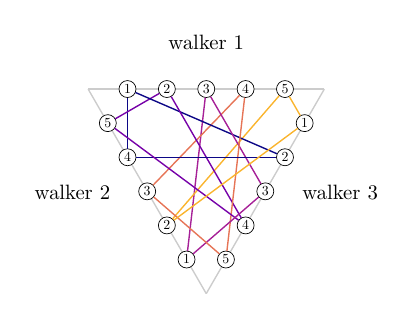
\begin{tikzpicture}
    \draw[color = black!20, line width = 0.5] (0,0) -- (\len,0);
    \draw[color = black!20, line width = 0.5] (0,0) -- ({\len*cos(60)},{-\len * sin(60)});
    \draw[color = black!20, line width = 0.5] (\len,0) -- ({\len*cos(60)},{-\len * sin(60)});

\node[draw, circle, scale = 0.65, fill = white, line width = 0.25](1) at ({\len / 6}, 0){};
\node[scale=0.5] at (\len / 6,0) {$1$};
\node[draw, circle, scale = 0.65, fill = white, line width = 0.25](2) at ({2 * \len / 6}, 0){};
\node[scale=0.5] at ({2 * \len / 6}, 0) {$2$};
\node[draw, circle, scale = 0.65, fill = white, line width = 0.25](3) at ({3 * \len / 6}, 0){};
\node[scale=0.5] at ({3 * \len / 6}, 0) {$3$};
\node[draw, circle, scale = 0.65, fill = white, line width = 0.25](4) at ({4 * \len / 6}, 0){};
\node[scale=0.5] at ({4 * \len / 6}, 0) {$4$};
\node[draw, circle, scale = 0.65, fill = white, line width = 0.25](5) at ({5 * \len / 6}, 0){};
\node[scale=0.5] at ({5 * \len / 6}, 0) {$5$};

\node[draw, circle, scale = 0.65, fill = white, line width = 0.25](6) at ({\len*cos(60) / 6}, {-\len * sin(60) / 6}){};
\node[scale=0.5] at ({\len*cos(60) / 6}, {-\len * sin(60) / 6}) {$5$};
\node[draw, circle, scale = 0.65, fill = white, line width = 0.25](7) at ({2*\len*cos(60) / 6}, {-2*\len * sin(60) / 6}){};
\node[scale=0.5] at ({2*\len*cos(60) / 6}, {-2*\len * sin(60) / 6}) {$4$};
\node[draw, circle, scale = 0.65, fill = white, line width = 0.25](8) at ({3*\len*cos(60) / 6}, {-3*\len * sin(60) / 6}){};
\node[scale=0.5] at ({3*\len*cos(60) / 6}, {-3*\len * sin(60) / 6}) {$3$};
\node[draw, circle, scale = 0.65, fill = white, line width = 0.25](9) at ({4*\len*cos(60) / 6}, {-4*\len * sin(60) / 6}){};
\node[scale=0.5] at ({4*\len*cos(60) / 6}, {-4*\len * sin(60) / 6}) {$2$};
\node[draw, circle, scale = 0.65, fill = white, line width = 0.25](10) at ({5*\len*cos(60) / 6}, {-5*\len * sin(60) / 6}){};
\node[scale=0.5] at ({5*\len*cos(60) / 6}, {-5*\len * sin(60) / 6}) {$1$};

\node[draw, circle, scale = 0.65, fill = white, line width = 0.25](11) at ({\len-(\len*cos(60) / 6)}, {-\len * sin(60) / 6}){};
\node[scale=0.5] at ({\len-(\len*cos(60) / 6)}, {-\len * sin(60) / 6}) {$1$};
\node[draw, circle, scale = 0.65, fill = white, line width = 0.25](12) at ({\len-2*(\len*cos(60) / 6)}, {-2*\len * sin(60) / 6}){};
\node[scale=0.5] at ({\len-2*(\len*cos(60) / 6)}, {-2*\len * sin(60) / 6}) {$2$};
\node[draw, circle, scale = 0.65, fill = white, line width = 0.25](13) at ({\len-3*(\len*cos(60) / 6)}, {-3*\len * sin(60) / 6}){};
\node[scale=0.5] at ({\len-3*(\len*cos(60) / 6)}, {-3*\len * sin(60) / 6}) {$3$};
\node[draw, circle, scale = 0.65, fill = white, line width = 0.25](14) at ({\len-4*(\len*cos(60) / 6)}, {-4*\len * sin(60) / 6}){};
\node[scale=0.5] at ({\len-4*(\len*cos(60) / 6)}, {-4*\len * sin(60) / 6}) {$4$};
\node[draw, circle, scale = 0.65, fill = white, line width = 0.25](15) at ({\len-5*(\len*cos(60) / 6)}, {-5*\len * sin(60) / 6}){};
\node[scale=0.5] at ({\len-5*(\len*cos(60) / 6)}, {-5*\len * sin(60) / 6}) {$5$};

\draw[color1,-,line width = 0.5] (1) -- (7);
\draw[color2,-,line width = 0.5] (2) -- (6);
\draw[color3,-,line width = 0.5] (3) -- (10);
\draw[color4,-,line width = 0.5] (4) -- (8);
\draw[color5,-,line width = 0.5] (5) -- (9);

\draw[color1,-,line width = 0.5] (1) -- (12);
\draw[color2,-,line width = 0.5] (2) -- (14);
\draw[color3,-,line width = 0.5] (3) -- (13);
\draw[color4,-,line width = 0.5] (4) -- (15);
\draw[color5,-,line width = 0.5] (5) -- (11);

\draw[color1,-,line width = 0.5] (12) -- (7);
\draw[color2,-,line width = 0.5] (6) -- (14);
\draw[color3,-,line width = 0.5] (10) -- (13);
\draw[color4,-,line width = 0.5] (8) -- (15);
\draw[color5,-,line width = 0.5] (9) -- (11);


\node[scale=0.75] at (\len / 2, \len / 5) {\lstinline{walker 1}};
\node[scale=0.75] at (-0.2, -\len *0.435) {\lstinline{walker 2}};
\node[scale=0.75] at (\len +0.2, -\len *0.435) {\lstinline{walker 3}};


\end{tikzpicture}